\chapter{Preliminaries}
\label{c2}

In this chapter we present background knowledge that is essential for a clearer understanding of the work presented in this thesis.
We introduce the research field of natural language processing (\as{nlp}) and detail its most common tasks.
Next, we clarify how computational text representation has shifted from simple high-dimensional binary vectors, that carry information if a specific word is within a text, to advanced representations based on real-number vectors that aim to represent the lexical meaning of words in a lower dimensional vector space.

Then, we describe what is information extraction detailing some of its major tasks, methods, and evaluation techniques commonly employed.
Finally, we reveal how biomedical text mining involves the application of \as{nlp} to extract information from text found in the scientific literature and electronic health records.
Related community-wide challenges and several biomedical resources are highlighted.

Some of the content presented in this chapter is based upon well-established literature, to which we point the reader for further consulting \parencite{manning2008a,bird2009a,nadkarni2011a,ingersoll2013a,jurafsky2018a}.


\section{Natural language processing}

Natural language processing, a subfield of artificial intelligence, investigates how a machine may `understand' natural language.
It includes a variety of text processing tasks, ranging from simpler exercises, such as finding the boundaries of sentences within a text, to more difficult challenges that can make machines answer questions, summarize or translate documents, or even maintain a human-like conversation.
Machines that can successfully address those more difficult \as{nlp} tasks are often referred to as `intelligent' because they show similar language reasoning abilities to those of humans.

To give some context, \textcite{turing1950a} defied the computational linguistics community by reformulating the question `Can machines think?' so that it could be expressed in a less ambiguous form.
The author further presented the \textit{imitation game} (also known as the \textit{Turing Test}) which, in short, is a simple assessment for evaluating if a machine can show intelligence similar to humans by communicating, as good as a human, through natural language (that is, if it is capable of imitating human answers).
Since then, a lot of research has been conducted regarding automatic (computational) processing of natural language---a very short historical roadmap about the field of \as{nlp} follows.

According to \textcite{nadkarni2011a}, \as{nlp} had its beginning around the 1950s with the intersection of the fields of artificial intelligence and linguistics.
\textcite{rindflesch1996a} presents a solid review of early \as{nlp} tasks that were solved using statistical techniques, probabilistic models, and rule-based approaches; and discusses some of the \as{nlp} applications such as information retrieval and question-answering systems.
According to \textcite{marquez2000a}, the application of machine learning drawn attention in the \as{nlp} community around the early 1990s addressing mainly natural language disambiguation.

However, in recent years deep learning has shown great promise in several computational research areas and \as{nlp} is no exception.
Deep learning--based strategies have established the state-of-the-art in many tasks achieving sometimes performance almost as good or better than a human.
Computational linguistics and deep learning have a huge potential that has been explored and there is still plenty room for investigation and future testing, with still much exciting experiments to offer \parencite{manning2015a}.

One of the most important applications of \as{nlp} in the biomedicine field is that these technologies help biologists, medical researchers, and physicians with tools that provide automatic annotation of text.
These are also fundamental for biocuration and help to keep biomedical databases and ontologies up-to-date \parencite{singhal2016b}.

In this section we detail the many tasks of \as{nlp} which deal with the basic processing of text. These are required to construct much more complex tasks such as those of information retrieval or extraction. These tasks are usually addressed using heuristics, rule-based approaches, or machine learning strategies.


\subsection{Tasks}

The field of natural language processing has many applications and it is in constant evolution with new use cases often emerging.
However, the main fundamental \as{nlp} tasks have remained essentially the same throughout the years.
Processing natural language usually consists in employing a variety of methods that solve simpler to more complex tasks, depending on the problem at hand.
The simpler, low-level, tasks constitute the main processing blocks, which are then used when addressing more complex, high-level, tasks.
We start by enumerating and briefly explaining some of the key \textit{lower-level} \as{nlp} tasks:

\begin{itemize}

\item
\textit{Sentence boundaries detection}, also referred to as \textit{sentence splitting}, is the task of identifying the boundaries of each sentence, that is, where sentences start and end.
It is relevant for further processing steps that take advantage of processing one sentence at a time.

\item
\textit{Tokenization} consists in splitting an excerpt of text into \textit{words}, though some specific tokenizers have a more granular approach and further split words into \textit{subword units}, also known in the literature as \textit{wordpieces}~\parencite{wu2016a}.
Each individual \mbox{(sub)}word is considered a \textit{token}.
Often this method is performed in a sentence (that is, after sentence splitting), though it can be applied in shorter phrases or longer excerpts such as a paragraph or a full-text document without sentence splitting.

\item
\textit{Stop words removal} discards words that may be considered noisy or irrelevant for a specific language understanding task.
Usually, pre-compiled lists of stop words, found in several \as{nlp} libraries and databases, are employed; though methods that dynamically identify the stop words are also used, for instance by finding highly frequent non-informative words in a collection of text documents (such as `the', `and', `or').
This technique is often employed for tasks such as document or topic classification, where main terms related to a certain topic contribute for a successful prediction.
For instance, \textcite{saif2014a} studied whether removing stop words is effective for sentiment analysis of Twitter posts.

\item
\textit{Stemming} and \textit{lemmatization} are two different techniques with the same goal, to convert or normalize related forms of a word to a common base form.
For example, \textit{activate}, \textit{activates}, and \textit{activating} could be chopped off to \textit{activat}.
This is what {stemming} performs, it employs a heuristic process that removes the ends of words (even if the resulting word form does not exist in the language).
One of the most known stemmers for the English language is the Porter stemmer \parencite{porter1980a}.
On the other hand, \textit{lemmatization} finds the root form of a word within a vocabulary corresponding to the base or dictionary form of a word, known as \textit{lemma} (usually a verb or a noun).
The resulting \textit{lemma} of the previous example would be \textit{activate} (verb) or \textit{activation} (noun).

\item
\textit{Part-of-speech tagging} consists in attributing to each word in a text its part-of-speech, that is, identifying whether its \textit{lexical category} is a noun, verb, adjective, or other.
These part-of-speech (\as{pos}) categories, also known as \textit{word classes}, are helpful for downstream tasks such as text chunking and named entity tagging.
Probably, the most well-known and established \as{pos} tagset for English is the one from the Penn Treebank Project\footnote{\url{https://www.ling.upenn.edu/courses/Fall_2003/ling001/penn_treebank_pos.html}} (1989--1992) which we point the reader for further consultation \parencite{santorini1990a,marcus1993a}.

\item
\textit{Text chunking} or \textit{shallow parsing} splits a sentence into contiguous and non-overlapping segments according to the part-of-speech tagged tokens.
Consecutive tokens are grouped into major grammatical units such as noun phrases, verb phrases, adjective phrases, and prepositional phrases.
Consult \textcite{abney1991a,sang1999a} for further reading.

\item
\textit{Dependency parsing} identifies the grammatical relations between words within a sentence, thus exposing its syntactic structure.
The relations are directed and labeled from a fixed set of grammatical relations or \textit{dependencies}, forming a structured tree of relationships known as \textit{dependency tree}.
The Stanford typed dependencies representation provides a standard description of grammatical relationships \parencite{marneffe2008a,marneffe2016a}, which was later extended and improved according to the Universal Dependencies representation \parencite{schuster2016a}.

\item
\textit{Passage segmentation} is responsible for finding and splitting the constituent sections of a full-text document.
Often a complete document contains several parts, and each of these sections may require a different text processing.
For example, in clinical reports, one section may have a list of medical prescriptions (with dosages, route of intake, and other relevant information), other section can contain a table with clinical analysis results, and other sections may simply have notes in raw text.

\item
\textit{Semantic role labeling}, also known as \textit{shallow semantic parsing} or \textit{slot-filling}, identifies semantic relationships, within a sentence, between noun and verb phrases with thematic roles such as \textit{agent}, \textit{instrument}, or \textit{destination} \parencite{gildea2000a,gildea2002a,jurafsky2018a}.
As \textcite{jurafsky2018a} further explain, this task aims to answer how participants relate to events addressing questions like ``who did what to whom'' and ``when and where''.

\end{itemize}


We have identified most of the major \textit{low-level} processing tasks of natural language, which are commonly employed in the implemententation of \textit{higher-level} tasks, that solve specific problems, such as:

\begin{itemize}

\item
\textit{Word sense disambiguation} aims to find the correct senses of ambiguous terms given their surrounding contexts. Natural language contains many equivocal expressions and frequently it is open to interpretation. Therefore, finding the proper meaning of ambiguous text is relevant for accurate information extraction.

\item
\textit{Named entity linking} or \textit{concept normalization} attributes unique identifiers---from databases, terminologies, or vocabularies---to terms identified in the text. Often, this task is tackled jointly with the sense disambiguation task because it requires linking every ambiguous expression to a unique meaning using a specific identifier.

\item
\textit{Document classification} consists in categorizing documents according to pre-defined criteria. For instance, documents can be classified within several topics or simply as relevant or not (example of binary classification).

\item
\textit{Named entity recognition} detects the spans of text that refer to specific entities (or concepts). For example in the biomedical domain, this task is used to detect diseases, adverse effects, chemicals, and others.

\item
\textit{Relation extraction} identifies interactions between named entities in the text. Traditionally, this task started by a \textit{trigger recognition} step where the term expression---usually a verb---involving the two entities would be firstly detected. However, with the recent advance of machine learning, this separate step for trigger recognition was discarded due to more recent \as{nlp} models that are able to perform relation extraction in a single step, usually through the use of distributed word representations.

\item
\textit{Text summarization} is the task of creating a short excerpt of a few sentences or paragraphs, given a larger input text, containing the most relevant information presented in the original document.

\item
\textit{Question answering} addresses the extraction or generation of textual answers to questions, which can be based on text data alone or by exploiting external information from knowledge sources.

\item
\textit{Machine translation} is the task of converting text in one language to another. For instance, given a clinical narrative in Spanish, transform it to English.

\end{itemize}

All the aforementioned \textit{higher-level} tasks are related to the broader concept of measuring the \textit{semantic textual similarity} between two text excerpts.
For instance, sense disambiguation and concept normalization compare the surrounding context of an ambiguous term to other contexts of other senses, identifying the \textit{closest} one and therefore the likely meaning.
Similarly, supervised relation extraction models identify interactions between two entities by using and \textit{interpreting} their surrounding context.


\section{Text representation}

Representing text in a numerical form is what allows mathematical models to be used for automatic processing of natural language.
Early approaches for text representation were based on binary vectors that indicated the presence or absence of a specific word from a determined vocabulary. These evolved to integer vectors that could tell how many times a word appeared in a text, and then more elaborated formulas appeared for giving a certain importance to each word.
One of the most fundamental \as{nlp} tasks is the splitting of the text into basic units such as words, also commonly referred to as tokens.
This process is known as tokenization and is the basis for representing the text.


\subsection{One-hot encoding and bag-of-words}

A simple way of thinking on how to convert a text document into a numerical representation is to simply attribute an integer number to each word in the vocabulary.
In this context, a vocabulary is the set of distinct words found in a collection of documents, or corpus.

One-hot encoding is a common technique for representing words using binary vectors.
First, the vocabulary is built, and the length of the vocabulary is considered the length of the binary vector.
Then, every word is attributed an integer number, corresponding to its index in the vocabulary, and a document is represented by a vector containing mostly zeros with ones indicating the words that are present in the document.

The bag-of-words (\as{bow}) technique consists in representing a text by specifying only its constituent words and their respective occurrence or frequency---their position in the text are ignored.
The most commonly used weighting scheme applied with \as{bow} is the \as{tf}--\as{idf} (term frequency--inverse document frequency).

The \as{tf}--\as{idf} mechanism has the goal to give higher importance to most common words within a document, but reduce importance to words that are frequent across the corpus.
For instance, considering the English language, words such as `the' and `of' are very frequent in a single document, but also in a set of documents, therefore carrying little information about a specific subject.

These techniques allow a simple and fast numerical representation of text that can achieve strong performances in several \as{nlp} tasks relevant for information extraction such as document classification.
In this case, each document corresponds to a vector where each dimension corresponds to a specific word, and its value can be the frequency count or the \as{tf}--\as{idf} value.
Commonly, this provides a solid baseline that can be used as a starting point for further development and improvement.
However, one drawback of this method is that does not benefit from the sequential order in which the words appear, that is, the real context and meaning of a structured sentence.


\subsection{Distributional semantics and word embeddings}

Distributed representations of words, also known as word embeddings, are lower-dimensional vector representations of words.
These are estimated from large corpora with millions or billions of words.
Although distributed word representations were proposed before, the first well-known algorithm for efficiently calculating these word embeddings is word2vec \parencite{mikolov2013b,mikolov2013a}, and then other models such as GloVe appeared \parencite{pennington2014a}.
These methods calculate fixed word vectors using deep learning models that during training try to predict the surrounding context given the target word, or try to predict the target word given the surrounding context.

These word vector representations are used frequently with deep neural network architectures.
An alternative type of representation is \textit{character embeddings} where each character is represented by a single vector.
These have been proven to be useful also for a variety of \as{nlp} tasks since these can encode and carry further information---for example they can retain information regarding prefixes and suffixes.


\section{Information extraction}

This section gives an overview of the \textit{Information Extraction} task.
It presents background work, state-of-the-art methods, and summarizes the description of many subtasks.
Within the text data mining field, information extraction is the process of using computerized and automatic methods to \textit{discover knowledge} from digital media sources such as textual data.
However, in a more broad sense, information extraction is often related with simply distilling data from document sources, and therefore, in fact, does not always imply \textit{discovering new knowledge}.

Arguably, the most addressed tasks for information extraction from free text are \textit{named entity recognition} and \textit{relation extraction}.
The former is responsible for identifying terms or concepts in the text, whereas the latter finds relationships between those concepts.
Automatic annotation of entities and their relations is relevant to generate new hypotheses that help to create new knowledge.
For instance, particularly within the biomedical domain, adverse drug events (\asp{ade}) can be determined, and candidate drugs or therapies for specific health problems can be detected from clinical reports.

The implementation of these tasks require the use of \as{nlp} methods which are able to handle and transform textual data.
These are usually employed in a first stage of data preparation for representing the text in a numerical form, which can then be interpreted by mathematical models such as machine learning methods.

Information extraction can be thought as the task of identifying relevant information in the text such as entity mentions and interactions (or relations) between those.
Linking (normalizing) entity mentions to standard terminologies or ontologies, or disambiguating them is also considered to be part of information extraction.
Classifying documents as pertinent to discover specific knowledge is also considered a relevant task for information extraction.

We also explain the basics of major NLP tasks including word sense disambiguation, document classification, entity recognition, and relation extraction.
Frequent methodologies including rule-based approaches, machine learning models, and deep neural networks are briefly introduced.
We also clarify different learning paradigms, used in information extraction, such as supervised, semi-supervised, distant supervision, unsupervised or knowledge-based, and explain how they make use of labeled and unlabeled data, and external information sources such as (curated) databases.
Additionally, we highlight the differences between pipeline and joint learning methods.
Concurrently, we present a brief overview of the biomedical information extraction research area, and detail further background work for different tasks in each chapter separately.


\subsection{Tasks}

There are a plethora of information extraction tasks.
In this section we highlight the ones that we considered more relevant according to the work developed for this thesis.
These primarily include the retrieval or classification of documents relevant for text mining, and further identification of named entities and their relationships.
These are the major steps required to help database curation and potentially find new hypotheses for testing.


\subsubsection{Document classification}

Document classification is the task of categorizing documents, for example by labeling them relevant or irrelevant regarding predefined criteria.
This task can be employed in an \as{ie} pipeline where the first step is to identify potentially relevant documents for text mining.
Document classification is sometimes interwoven with document retrieval, where a large collection of documents is present, and the most relevant regarding a specific subject need to be selected; in these case, the advantage is that only a smaller subset of documents needs to be processed with further \as{ie} tasks, alleviating the need of computational power.


Earlier approaches for classifying documents included rule-based methods built with heuristics.
Though, with the increasing of hand-labeled data, traditional supervised machine learning methods started to be applied using bag-of-words features.
Most recent works have been using deep learning architectures with word embeddings for text classification \parencite{yang2016a,fergadis2018a}.
These methods have been applied for a variety of purposes including finding depressive tendencies in written text \parencite{yates2017a} and performing sentiment analysis \parencite{cambria2013a}.

Classification of documents can expedite next information extraction steps since irrelevant, or less relevant, documents can be discarded beforehand.
The removal of this unnecessary texts saves valuable processing time that can be employed for more important tasks such as finding relationships between relevant terms.
However, the document classification task may not be necessary when it is the aim---and there is enough computational power---to analyze all the documents of a collection, or the number of documents is relatively small.


\subsubsection{Named entity recognition}

Named entity recognition (\as{ner}) is a major task in information extraction from text.
Its aim is to identify named entities such as persons, organizations, locations in the case of general-domain text; or chemicals, diseases, and adverse drug effects in the case of biomedical text.
This is the most fundamental task for enabling relationship extraction between the pre-detected named entities.
For example, considering biomedical text, chemical--protein or drug--drug interactions  can be found, and verified or added to external databases by expert curators.

Earlier approaches for \as{ner} were based on machine-readable dictionaries (\asp{mrd}) that contain lists of entity terms of different types.
This strategy constitutes one of the most simple method for entity recognition, since it is only required to match the entity terms within the text---for that case, regular expressions can be used.
Regular expression is a method that facilitates the programming of finding text patterns in a concise way, and it has been used for several years in many text processing related areas.

Afterwards, named entity recognition was addressed as a sequence labeling problem, where each token is labeled as part of an entity or not.
This is the most common way to solve \as{ner}, since it provides a simple way for detecting the entity boundaries (character offsets), and classify the entity type if it is the case of multiple entity classes.
Conditional random fields (\asp{crf}) are statistical models that have been largely used in natural language processing.
These do not predict the label of each token independently, but take context (neighboring tokens) into account.

To the best of our knowledge, \textcite{ramshaw1995a} proposed the \{I, O, B\} chunk tag set when implementing a rule-based tagging system for text chunking.
In their work they used the ``I'' tag to mark words inside some noun phrase~(\as{np}), the words marked with ``O'' are outside the \as{np}, and the ``B'' tag is used to mark the first word of a \as{np} which immediately follows another \as{np}.

However, different representations for chunking and named entity recognition~(\as{ner}) have been proposed and been used as well.
For instance, \textcite{sang1999a} examined seven different representations for the problem of recognizing \as{np} chunks, where they cite the work of \textcite{ratnaparkhi1998a} highlighting that in his work all the chunk initial words receive the same start tag differently from the representation used by \textcite{ramshaw1995a}.
\textcite{sang1999a} refer to the tagging formats proposed by \textcite{ramshaw1995a} and \textcite{ratnaparkhi1998a} as ``IOB1'' and ``IOB2'' respectively.
They also present the ``IO'' partial representation in which words inside a \as{np} receive an ``I'' tag and others receive an ``O'' tag.
However, this encoding is insufficient since adjacent \asp{np} or named entities cannot be distinguished.

In the \as{ner} task across multiple domains, \textcite{ratinov2009a} found that the \as{bilou} (also known as IOBES) representation of text chunks significantly outperforms the widely adopted IOB scheme.
In the biomedical domain, \textcite{dai2015a} studied the effect of different tagging schemes showing that the IOBES scheme obtained better results than the IOB scheme in the recognition of mentions of chemical entities.
However, in another work in \as{ner}, \textcite{lample2016a} did not observe a significant improvement of the IOBES tagging scheme over the IOB tagging scheme.

\begingroup
% \normalfont
% \color{black}

\begin{table}[!t]

\caption{Tagging schemes, their nomenclatures and abbreviations.}
\label{tab:tagging-schemes}

\centering
% \small

\begin{tabular}{lll}

\toprule

Nomenclatures & Initials & Meanings\\

\midrule

\multirow{2}{*}[-0pt]{IO} & I & Inside\\

& O & Outside\\

\midrule

& I & Inside\\

IOB, BIO & O & Outside\\

& B & Beginning\\

\midrule

& I & Inside\\

& O & Outside\\

IOBES, BILOU & B & Beginning\\

& E / L & End / Last\\

& S / U & Single / Unit-length\\

\bottomrule

\end{tabular}
\end{table}
\endgroup


Different names for the same tagging schemes have been used.
\Cref{tab:tagging-schemes} presents an incomplete list of these nomenclature variations and their abbreviations.
For more details, we point the reader to other works reporting investigation of different tagging schemes \parencite{kudo2001a,cho2013a}.
An example, adapted from \textcite{cho2013a}, with the use of the ``IO'', ``IOB2'' and ``IOBES'' representations is shown in \Cref{tab:tagging-schemes-example}.

\begingroup
% \normalfont
% \color{black}

\begin{table}[!t]

\caption[A sample text annotated with different tagging schemes.]{A sample text annotated with different tagging schemes. Adapted from \textcite{cho2013a}.}
\label{tab:tagging-schemes-example}

\centering
% \small

\begin{tabular}{llll}

\toprule

Tokens & IO & IOB2 & IOBES\\

\midrule

Gamma & I-gene & B-gene & B-gene\\

glutamyl & I-gene & I-gene & I-gene\\

transpeptidase & I-gene & I-gene & E-gene\\

( & O & O & O\\

GGTP & I-gene & B-gene & S-gene\\

) & O & O & O\\

activity & O & O & O\\

in & O & O & O\\

the & O & O & O\\

... & ... & ... & ...\\

\bottomrule

\end{tabular}
\end{table}
\endgroup



\subsubsection{Named entity linking}

Named entity linking, or entity normalization, is the task of attributing unique codes from standard terminologies to the previously detected entity mentions.
This step is usually performed after the named entity recognition task, where entities are predicted, but are not linked to a curated ontology or database.
This task also addresses word sense disambiguation (\as{wsd}), since it is guaranteed that every entity mention has a specific meaning because it is connected to a single code.

The task is usually solved using sieve-based approaches, where in each sieve (step) it is performed a different strategy.
It is common that the first sieves are based on string matching patterns using dictionaries from standard terminologies, followed by more advanced techniques for example including measuring similarities using word embeddings.
The resolution of this task is relevant since it helps in the relationship extraction task, and guarantees exactly which concepts are being referred, which is important for accurate information extraction.


\subsubsection{Relation extraction}

Relation extraction (\as{re}) or relationship extraction aims to identify associations between specific entities in the text.
This task commonly follows the entity recognition task where named entities are firstly properly identified.
The relations detected and discovered are then relevant to help curators keep their databases well-verified and up-to-date.

Traditionally this task started with the identification of a trigger for a relation.
This is known as trigger recognition, where for example a verb could identify the relation between two concepts.
\textcite{campos2014a} present a machine learning model for biomedical event trigger recognition. They use a \as{crf} with a comprehensive feature set achieving an F-score of 0.627 in the \as{bionlp} 2009 shared task corpus.


\subsection{Pipelined \versus\ joint extraction}

Traditionally, extraction of entities and relations have been addressed by solving two ordered tasks: \as{ner} and relation extraction. This is commonly referred in literature as the \emph{pipeline} approach, since it combines two separate tasks where the relation extraction requires beforehand the named entities.

There are two main paradigms for extracting information:

\begin{itemize}
\item
Pipelined: concept recognition followed by relation extraction.
\item
Joint extraction where entities and relations are simultaneously extracted.
\end{itemize}


\subsubsection{Pipelined extraction}

Pipelined extraction is built with two separate steps: named entity recognition is followed by relation extraction. In this approach, these steps require training two different models.
One weakness of this approach is that the \as{ner} step can propagate errors into the last step \parencite{li2014b}.


\subsubsection{Joint extraction}

Joint extraction is the task of cooperatively identifying entities and their semantic relations from free text.
Traditional joint methods require complex feature engineering or heavily rely on other \as{nlp} tools. However, the use of external tools might lead to error propagation where wrongly detected named entities negatively impact the relation extraction task.
In recent years, the use of neural networks (deep learning) has been investigated for developing end-to-end models dramatically reducing the manual effort in feature extraction.

In this section we present works that either apply feature-engineered or deep learning methods, discussing what are the conveniences over each other.


\paragraph{Handcrafted feature engineering}

First works on joint extraction were built with two separate models, where one was responsible for \as{ner} and the other performed relation extraction.
Afterward, works using only a single joint model were proposed.
To the best of our knowledge, \textcite{li2014b} were the first to present a single joint model to predict entities mentions and relations.
The entity and relation extraction tasks they addressed were those of the Automatic Content Extraction~(\as{ace}) program \parencite{doddington2004a} presenting results on the \as{ace}04 and \as{ace}05 corpora.
In contrast to previous research where entity mentions are assumed to be given, this work aimed to investigate an end-to-end model for \as{ner} and relation extraction.
For comparison, they developed a baseline pipeline system composed of a \as{crf} for entity mention extraction and a maximum entropy model for relation extraction.
In the \as{ace}04 corpus their joint model achieved a 0.453 F1-score outperforming previous works and their pipeline baseline model (0.429).
In the \as{ace}05 corpus their proposed joint model achieved a 0.495 F1-score, whereas human annotators obtained an F1-score about 0.70 with an inter-annotator agreement of 0.519, showing how end-to-end relation is challenging.

\textcite{miwa2014a} introduced a flexible table representation of entities and relations from a single sentence.
They employed the \as{bilou} tagging scheme assuming that entities do not overlap.
They evaluated their model in the \as{conll}04 dataset \parencite{roth2004a}.
Their F1-score metrics showed improved performance in using joint learning (0.610) over a pipeline approach (0.577).

\textcite{ren2017a} combined joint extraction of entities and relations with distant supervision. They evaluated their model in three datasets from different domains (news articles, Wikipedia articles, biomedical abstracts).


\paragraph{Deep learning}

\textcite{miwa2016a} presented the first neural network based model for joint extraction of entities and relations.
Their end-to-end model represents word sequence and dependency tree structures by using bidirectional sequential and tree-structured \as{lstm} (long short-term memory) networks. In the \as{ace}04 and \as{ace}05 datasets they achieved F1-scores of 0.484 and 0.556 respectively.

\textcite{katiyar2017a} employed an attention-based \as{bilstm} model for joint entity and relation extraction.
They made no use of dependency trees neither \as{pos} tags, using only the surface form (sequence of tokens) and achieved competitive results compared to the previous work of \textcite{miwa2016a}.

\textcite{zheng2017a} proposed a novel tagging scheme for jointly extracting entities and relations.
Their tagging scheme expands the \as{bilou} scheme.
Besides each token's tag having associated information about its position within an entity, it also contains information about the relation and if it is the first or second entity in a triplet.
Their end-to-end model, based on \as{lstm} networks, achieved the best results for a dataset created by distant supervision means \parencite{ren2017a}.
However, their method cannot handle overlapping relations.

\textcite{li2017a} presented another neural joint model.
They evaluated their model in two tasks: the task of extracting \asp{ade} between drug and disease entities, and the task of extracting resident relations between bacteria and location entities.
They used parameter sharing to join two \as{bilstm} networks for extracting entities and relations.
They used the \as{bilou} labeling scheme for entity recognition.

\textcite{adel2017a} applied global normalization of convolutional neural networks.
Following \textcite{miwa2014a}, and \textcite{gupta2016a} they tackled the problem as a table filling task and did not require to transform it into a token-labeling problem.

\textcite{zheng2017c} proposed a hybrid neural network composed of a \as{lstm} for entity extraction and a \as{cnn} (convolutional neural network) for relation classification.
However, the first layer is a \as{bilstm} encoding layer which is shared for both tasks.
They evaluated their model in the \as{ace}05 dataset surpassing previous works.

\textcite{verga2018a} proposed a bi-affine relation attention network that simultaneously extract relations at the document-level.
They also employed strong distant supervision to create a new dataset, from \as{pubmed} abstracts and the Comparative Toxicogenomics Database (\as{ctd}), for biological relation mining (chemical-disease, chemical-gene, gene-disease).

\textcite{bekoulis2018c} demonstrated that the use of adversarial training, by adding noise to the word representations, improves joint extraction of entities and relations from datasets of different domains.
Moreover, their model with adversarial training achieved high performance in the first epochs during the training process.

\textcite{bekoulis2018a} employed a \as{bilstm} encoding layer, a \as{crf} for entity recognition, and a sigmoid function for relation extraction.
They conducted a large scale experiment achieving state-of-the-art results in corpora from different domains (news, biomedical, real estate) and languages (English, Dutch).

More recently, \textcite{eberts2019a} proposed a span-based joint entity and relation model that uses as its core a pre-trained \as{bert} (bidirectional encoder representations from transformers) network~\parencite{devlin2019a}.
Their span-based approach considers that any token subsequence is a potential entity, and that any pair of spans can have a relation.
A full search over all span and relation candidates is performed.
They claim that one advantage of this approach over the use of \as{bio} or \as{bilou} tagging schemes is that it can identify overlapping entities (for example, ``codeine'' within ``codeine intoxication'').
In their relation classifier they considered the context between the two entities, since it showed to be more profitable than using the whole sentence.
They reported state-of-the-art results in three datasets: \as{conll}04, SciERC \parencite{luan2018a}, and \as{ade} \parencite{gurulingappa2012a}.

\textcite{wadden2019a} followed the work of \textcite{luan2019a} additionally performing event extraction, and building span representations on top of multi-sentence \as{bert} encodings.
They experimented on four datasets: \as{ace}05, SciERC, GENIA \parencite{kim2003a} and \as{wlpc} \parencite{kulkarni2018a}.

\textcite{luo2020a} proposed a new tagging scheme to represent both entities and relations.
Their scheme can represent some overlapped relations, which provides better performance in comparison to other works.
They employ a \as{bilstm}-\as{crf} model with an attention mechanism.
They also had to define their own extraction rules according to the proposed scheme.


\subsection{Methods}

There are a variety of methods for extracting information.
Earlier methods were built manually implementing handcrafted rules.
Then, rule-based and knowledge-based methods followed.
And during the past years, due to the the much-higher availability of computational power and also labeled text data, machine learning methods started to thrive, particularly deep learning models that perform better with large amounts of data.

Handcrafted rules are usually constructed using if-else statements or using regular expressions that can find patterns in text.
This approach is usually efficient in terms of computational performance, but requires some expertise in the field for constructing these rules, and the accuracy results may not be the best.

Traditional machine learning models also have had great success for document classification, entity recognition, and relation extraction.
These models include kernel classifiers such as support vector machine, k-neighbors classifier, decision tree, and probabilistic methods such as the Naive Bayes classifier.

Due to the access to big data, and increasingly gold-standard labeled data, deep learning models have been successfully claiming the state-of-the-art for many language processing tasks.
Deep models include convolutional and recurrent neural networks, attention mechanisms, generative adversarial networks, and transformers.


\subsubsection{Machine learning}

Machine learning models are based on statistical and probabilistic methods that make use of training data to \textit{learn} a specific task.
These are used for building robust predictive systems in different scenarios and applications including computer vision and speech recognition, though in here we briefly present only some of the most known or used methods applied in natural language processing.


\paragraph{Naive Bayes}

This is known to be a straightforward classifier based on a probabilistic method, which has worked well in many different data mining tasks including document classification.
These models are much faster compared to more complex methods, and usually do not require large amounts of training data.


\paragraph{k-nearest neighbors}

This classifier is often used as a solid baseline classifier in many different machine learning tasks.
It also provides a robust approach for a variety of \as{nlp} problems including document classification.
It follows a simple algorithm where a sample is classified as the majority vote of its neighbors.
That is, if the majority of the nearest points in the space are from a specific class, then the sample will have this class as prediction.
This method is also straightforward and fast to compute, and does not require much training data for reasonably good results.


\paragraph{Decision tree}

This classifier is also a simple algorithm yet effective in a variety of tasks also providing a solid baseline for machine learning problems.
It works by building a flowchart-like, from the root node to low-level nodes, with consecutive binary decisions according to the values of the features.
The more depth the tree, the more complex, questions become more refined, which may provide better results or overfit to the training data if there is excess `memorization' on noisy patterns of the data.


\paragraph{Support vector machine}

This model is one of the most used in traditional machine learning, and often provides strong results.
This classifier tries to separate training examples from different classes by maximizing their distance in the space.
New samples are then predicted according to which side they belong to.
\asp{svm} are efficient when dealing with high-dimensional feature spaces.


\paragraph{Conditional random field}

\textcite{lafferty2001a} proposed the conditional random field model which has been used in computer vision and natural language processing for sequence labeling problems.
During the last years, these models combined with \asp{lstm} have been achieving state-of-the-art results \parencite{lample2016a}.


\subsubsection{Deep learning}

Deep learning has been an emerging \as{ai} research area in the last years, being considered a subfield of machine learning.
It is related with the use of (deep) neural network models for machine learning tasks.
Neural network models, built primarily from simple math-operation cells (neurons), were inspired from the human brain structure and have been researched during the last decades \parencite{hinton1992a}.
However, in the last years they have shown greater performance due to improved training methodologies, increased computational power, and higher availability of labeled data for training.

The most common and standard neural network, also known as multi-layer perceptron (\as{mlp}), is composed of one input layer and one output layer, and can have multiple intermediate (hidden) layers.
If there is at least one hidden layer then the model is considered to be a \textit{deep neural network}---hence the term \textit{deep learning}.
Each layer of the network can have multiple neurons increasing the model's complexity.

Other type of neural networks were then proposed and are specialized in different tasks.
Convolutional neural networks containing convolutional layers are mostly used in image processing, whereas recurrent neural networks that contain a feedback loop are used for text processing tasks.
These different networks can combine the input features in different ways and create robust representations of the input data allowing these models to perform well in supervised learning settings.


\subsubsection{Knowledge-based}

Knowledge-based methods are similar to unsupervised methods because they do not rely on gold-standard labeled training data.
However, these methods make use of external knowledge present in curated databases, terminologies, ontologies, or other types of information sources.
Strategies based on external knowledge have the objective to infer or predict new information by finding similarities with the currently known associations.


\subsection{Learning paradigms}

There are different learning paradigms when implementing automatic methods for information extraction.
Knowledge-based methods rely on external knowledge resources to empower their decision ability.
In machine learning it is common to consider three major learning paradigms: supervised, semi-supervised, and unsupervised.
Supervised algorithms require labeled training data to train and teach machine learning models what is what.

Information extraction frequently aims to extract specific and pre-specified relations from homogeneous data, such as for example, extracting adverse drug events from medical records.
In contrast, extracting relations from distinct domains is difficult since it requires to create new handcrafted rules or to annotate new training samples for being used in a supervised setting.
To alleviate this issue by facilitating domain-independent relation extraction from large and varied corpora as the Web, \textcite{banko2007a} introduced a new extraction paradigm, open information extraction~(\as{oie}), where the proposed system \enquote{makes a single data-driven pass over its corpus and extracts a large set of relational tuples without requiring any human input.}
As stated by \textcite{banko2007a}:

\blockquote{%
Standard \as{ie} systems can only operate on relations given to it \apriori\ by the user, and are only practical for a relatively small number of relations.
In contrast, open \as{ie} operates without knowing the relations \apriori, and extracts information from all relations at once.
}

They proposed a system for automatically extracting possible relations of interest.
Their system is composed of three steps: (1) a self-supervised learner that uses a naive Bayes~(\as{nb}) classifier and heuristics based on the dependency parsing, (2) a single-pass extractor that tags each word with its part-of-speech~(\as{pos}) and it finds relations between noun phrases~(\asp{np}), and (3) a redundancy-based assessor that creates normalized forms of the relations which are used to count the number of distinct sentences from which each relation was found.

Open \as{ie} systems have been used in several natural language processing~(\as{nlp}) tasks and these are traditionally built using patterns.
Some of its applications are question answering \parencite{fader2014a}, relation extraction \parencite{soderland2010a,fader2011a} and information retrieval \parencite{etzioni2011a}.

Despite these open \as{ie} systems being useful for extracting many generic relations, this is not the case when finding specific biomedical relations such as \asp{ade} or protein-protein interactions~(\asp{ppi}).
These type of biomedical relations are harder to extract since they contain specific vocabulary, and in the special case of using clinical reports there are usually many abbreviations and misspelling words increasing the level of ambiguity.
Commonly, small datasets with hundreds or thousands of documents are automatically collected using precise queries and manually annotated with these narrow type of relations for empowering the evaluation of biomedical text mining systems.


\subsubsection{Supervised}

Supervised learning is a strategy that uses gold-standard labeled training data to train machine learning models.
These models learn from ground-truth examples and, after being trained, they can identify and distinguish previously seen patterns on new different data.
This technique is often the one that performs best, but has the limitation that usually requires large amounts of high-quality training data.
And the manual process of expert annotation of data is very burdensome and expensive.


\subsubsection{Unsupervised}

Unsupervised learning algorithms have the objective to find patterns from unlabeled data.
The idea is that the model is able to create compact internal representations of the data, and then differentiate distinct features.
Approaches used in unsupervised learning include probabilistic methods (algorithms such as clustering) and neural networks.


\subsubsection{Semi-supervised}

Semi-supervised learning lies between the two extremes of learning paradigms, that use no labeled data (unsupervised) or only use labeled data (supervised).
This technique often consists in using a small set of gold-standard labeled training data, and the remaining training data is usually labeled by an heuristic method or with the help of an existing knowledge base.
The advantage of these strategies is that they require a lesser amount of curation work for creating ground-truth annotations.


\paragraph{Distant supervision}

To the best of our knowledge, the first use of learning from weakly labeled data in the biomedical domain was employed by \textcite{craven1999a} to construct knowledge bases for molecular biology, where they exploited databases to automatically label training instances.
They present a method to represent unstructured natural language text, from the \as{medline} biomedical scientific literature, into a structured form such as a knowledge base or a database.
As \textcite{craven1999a} state:

\blockquote{%
Our approach is motivated by the observation that, for many \as{ie} tasks, there are existing information sources (knowledge bases, databases, or even simple lists or tables) that can be coupled with documents to provide what we term ``weakly'' labeled training examples.
We call this form of training data weakly labeled because each instance consists not of a precisely marked document, but instead it consists of a fact to be extracted along with a document that \emph{may} assert the fact.
}


\subsection{Evaluation metrics}

In order to measure the performance of an \as{ie} system, specific metrics are usually employed to measure the quality of the predicted annotations \parencite{chinchor1993a,fawcett2006a,dalianis2018a}.
In this calculation, the predicted annotations are compared with the gold-standard annotations commonly made by expert curators.
Predicted annotations are considered true if they strictly match the gold-standard annotations, and false otherwise.
Furthermore, system predictions can be positive if the system provides an annotation (for example, it identifies a chemical entity mention in a text), or negative if the system does not provide any annotation (for example, no chemical entity mention is found).
Therefore, predictions can take one of distinct four classes (\Cref{fig:evaluation}):

\begin{itemize}

\item
True Positive~(TP): correct prediction, the annotation exists in the curated corpus;

\item
False Positive~(FP): incorrect prediction, the annotation does not exist in the curated corpus but the system predicted it;

\item
True Negative~(TN): correct prediction, the annotation does not exist in the curated corpus;

\item
False Negative~(FN): incorrect prediction, the annotation exists in the curated corpus but the system did not predict it.

\end{itemize}

% \FloatBarrier
\begin{figure}[!t]
\begin{center}
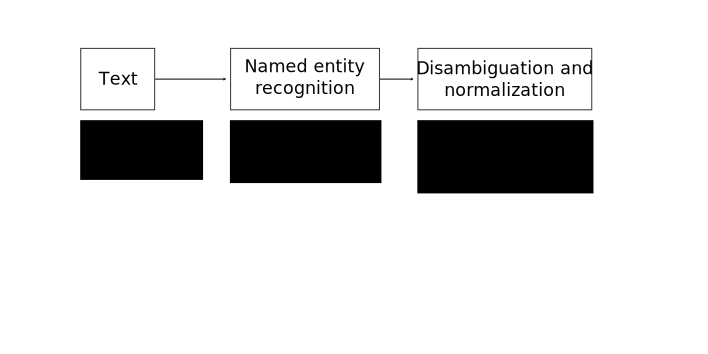
\includegraphics[width=\textwidth]{img/evaluation/v6/img.pdf}
\caption[Spatial visualization of true (false) positives and true (false) negatives.]{Spatial visualization of true (false) positives and true (false) negatives. Image adapted from \url{https://en.wikipedia.org/wiki/Precision_and_recall}.}
\label{fig:evaluation}
\end{center}
\end{figure}
% \FloatBarrier


In this scenario, the used metrics to evaluate the classification problem are Precision, Recall, Accuracy, Specificity, and F1-score.
These metrics assume values between zero, in the worst case, and one, in the best case.

Precision is the ratio between the number of true positives and the number of positive predictions.
In contrast, recall or sensitivity is the ratio between the number of true positives and the number of positive curated annotations.
Accuracy is the ratio between the correct (positive or negative) predictions and the total number of (positive or negative) predictions.
Specificity is the ratio between the number of true negatives and the number of negative curated annotations.
F1-score, or F1-measure, is the harmonic mean of precision and recall.
These metrics are shown in \Cref{eq:precision,eq:recall,eq:accuracy,eq:specificity,eq:f-score}.

\begin{equation}
\label{eq:precision}
\Precision = \frac{\TP}{\TP + \FP}
\end{equation}

\begin{equation}
\label{eq:recall}
\Recall = \frac{\TP}{\TP + \FN}
\end{equation}

\begin{equation}
\label{eq:accuracy}
\Accuracy = \frac{\TP + \TN}{\TP + \TN + \FP + \FN}
\end{equation}

\begin{equation}
\label{eq:specificity}
\Specificity = \frac{\TN}{\TN + \FP}
\end{equation}

\begin{equation}
\label{eq:f-score}
\Fscore = 2 \cdot \frac{\Precision \cdot \Recall}{\Precision + \Recall}
\end{equation}

~

In diverse information extraction and \as{nlp} tasks such as document classification, named entity recognition, and relation extraction, the most used metrics are precision, recall, and F1-score.
Particularly, in multi-class classification problems that deal with the prediction of multiple classes---for example, multiple document topics, entity or relation types---it is common to consider specific different averaging formulas for taking into account the individual performance for every class.
These are known as \textit{macro-average} and \textit{micro-average} \parencite{yang1999a,tsoumakas2009a}.
Macro-averaging consists in first calculating the score for every class and then averaging the per-class scores to obtain the final macro-averaged score.
On the other hand, micro-averaging consists in first summing up the number of true (false) positives (negatives) of every class, and then calculate the micro-averaged score using these global counts.
Curiously, \textcite{opitz2019a} present two slightly different ways of calculating the macro-averaged F1-score, but conclude that the commonly employed formula---average of F1-scores per each class---is the more robust.


\section{Biomedical text mining}
\label{c2:s:biomedical-text-mining}

In this section we present background material about \as{nlp} applied in the biomedical domain.
In the biomedicine research field, new concepts are discovered regularly and their term expressions are added to the current biomedical vocabulary.
Therefore, it is of utmost importance to keep standard terminologies, vocabularies, and databases updated with biological and medical curated information.
We present (1) several resources, such as databases and thesauri, that are commonly used in biomedical information extraction pipelines, and (2) worldwide shared-tasks and challenges aiming to improve biomedical text mining systems.

Biomedical information extraction is concerned with the understanding of natural language texts in the biomedical domain, and has the objective of mining information from these unstructured textual data and represent them in a structured and unambiguous way.
Due to the enormous quantity of biomedical information registered in textual form, such as scientific documents or clinical health records, it is impractical to manually acquire and link all the existing knowledge \parencite{cases2013a}.
Therefore, automatic \as{ie} and text mining solutions are helpful for integrating current biomedical information \parencite{krallinger2005a,ananiadou2006a}.


\subsection{Resources}
\label{c2:ss:resources}

Biomedical text mining is achievable due to the large number of resources that are available \parencite{simpson2012a,rebholzschuhmann2012a,zhu2013a,przybyla2016a,rosarioferreira2021a}.
Artificial intelligence--based techniques, such as machine learning and knowledge-based methods, rely on training or external data for extracting information from free text.
It is due to the manual curation efforts of biomedical experts that nowadays there is a large amount of standard datasets for biomedical \as{ie} tasks and other well-established sources of information such as databases and terminologies.
Biomedical curated data store biomedical knowledge that is essential for building text mining systems, and these data resources can be mainly split into two distinct groups:

\begin{itemize}

\item
\textit{Corpora} are collections of annotated documents that are used for assessing and comparing different \as{ie} solutions.
For instance, these documents may contain annotations about concepts and their relationships that are previously annotated by expert curators.

\item
\textit{Knowledge bases} are repositories that collect information with the goal of modeling the behavior and reality about some field.
Databases and ontologies are two types of knowledge bases.
While databases are restrictively a structured collection of data (tables, schemes), ontologies are more rich since they also interconnect the data (graphs, tree structures).
The type of knowledge base to be used should be chosen accordingly with the user needs, since ontologies are considered better than databases for representing domain concepts with higher level of detail, but databases may be more efficient \parencite{martinezcruz2012a}.

\end{itemize}

Aside from these data resources, other materials relevant to the development of biomedical text mining systems include:

\afterpage{
\begingroup
% \normalfont
% \color{black}
\singlespacing

% \renewcommand{\arraystretch}{1.2}
\setlength\tabcolsep{4.0pt}

% \newcommand{\z}{\hspace*{1em}}
\newcommand{\minorfootnotesize}{\fontsize{9.7pt}{11.64pt}\selectfont}

\small
% \footnotesize
% \scriptsize
% \minorscriptsize
% \tiny

% O   + E    + I*2    + E
% 0.0 + 0.38 + 0.02*2 + 0.58 = 1.0

% \begin{longtable}[c]{OE{0.38\textwidth}IIE{0.58\textwidth}N}
\begin{longtable}[c]{E{0.29\textwidth}p{0.67\textwidth}}

\caption{A list of biomedical databases, ontologies, and terminologies.}
\label{tab:biomedical-databases}\\

\toprule

Resource & Description\\
% \textbf{Resource} & \textbf{Description}\\

\midrule

\as{biogrid}\newline{\footnotesize\parencite{chatraryamontri2017a}} & Biological General Repository for Interaction Datasets (\as{biogrid}) is a database containing protein, genetic, and chemical interactions.\newline{\minorfootnotesize\url{https://thebiogrid.org}}\\

\midrule

\as{ctd}\newline{\footnotesize\parencite{davis2017a}} & Comparative Toxicogenomics Database (\as{ctd}) contains information about interactions between chemicals, genes, and diseases.\newline{\minorfootnotesize\url{https://ctdbase.org}}\\

\midrule

DrugBank\newline{\footnotesize\parencite{wishart2018a}} & DrugBank is a database containing molecular information about drugs, their mechanisms, interactions, and targets.\newline{\minorfootnotesize\url{https://www.drugbank.com}}\\

\midrule

\as{mesh}\newline{\footnotesize\parencite{lipscomb2000a}} & Medical Subject Headings (\as{mesh}) is the terminology used for indexing articles for \as{medline} literature.\newline{\minorfootnotesize\url{https://www.ncbi.nlm.nih.gov/mesh}}\\

\midrule

\as{mimic}-III\newline{\footnotesize\parencite{johnson2016a}} & Medical Information Mart for Intensive Care (\as{mimic}) is a large database comprising information, such as medications and clinical notes, about patients admitted to critical care units.\newline{\minorfootnotesize\url{https://mimic.mit.edu}}\\

\midrule

\as{obo} Foundry\newline{\footnotesize\parencite{smith2007a}} & The Open Biological and Biomedical Ontologies (\as{obo}) Foundry is an initiative for maintaining a family of interoperable ontologies in the biomedical domain.\newline{\minorfootnotesize\url{https://obofoundry.org}}\\

\midrule

\as{pubmed}\newline{\footnotesize\parencite{sayers2021a}} & \as{pubmed} (Public \as{medline}) is a database comprising scientific abstracts and citations published in life science journals.\newline{\minorfootnotesize\url{https://pubmed.ncbi.nlm.nih.gov}}\\

\midrule

\as{snomed}\newline{\footnotesize\parencite{cornet2008a}} & Systematized Nomenclature of Medicine (\as{snomed}) is a global standard for clinical health terminology.\newline{\minorfootnotesize\url{https://www.snomed.org}}\\

\midrule

\as{umls}\newline\footnotesize{\parencite{mccray1989a}} & Unified Medical Language System (\as{umls}) integrates biomedical terminology, coding standards, and other resources such as a semantic network for improving interoperability between biomedical information systems.\newline{\minorfootnotesize\url{https://www.nlm.nih.gov/research/umls/index.html}}\\

\midrule

\as{uniprot}\newline\footnotesize{\parencite{theuniprot2017a}} & Universal Protein Resource (\as{uniprot}) is a repository containing information about protein sequences and associated information.\newline{\minorfootnotesize\url{https://www.uniprot.org}}\\

\bottomrule

\end{longtable}
\endgroup
}


\begin{itemize}

\item
\textit{Toolkits and frameworks} enable a fast and easier prototyping of more complex \as{nlp} architectures.
Examples include \as{nltk} \parencite{loper2002a}, \as{ctakes} \parencite{savova2010a}, Gensim \parencite{rehurek2010a}, and Flair \parencite{akbik2019a}.

\item
\textit{Annotation tools and applications} provide a medium to aid domain experts manually annotate documents \parencite{neves2021a}.
Examples include \as{brat} \parencite{stenetorp2012a}, MyMiner \parencite{salgado2012a}, PubTator \parencite{wei2013b}, and LitSuggest \parencite{allot2021a}.

\item
\textit{Standard formats for interoperability}, such as BioC \parencite{comeau2013a}, easen the processing of distinct annotated datasets by different \as{nlp} systems.

\item
\textit{Pre-trained models} are usually made publicly available to allow reuse, evaluation, and reproducibility by other researchers.
These include, for example, word and sentence embeddings such as BioWordVec \parencite{zhang2019c} and BioSentVec \parencite{chen2019g}, and contextualized word representation models such as BioBERT \parencite{lee2020a} and PubMedBERT \parencite{gu2021a}.

\end{itemize}

\Cref{tab:biomedical-databases} presents some publicly available databases, ontologies, and terminologies that are relevant in the biomedical domain and useful for supporting the construction of biomedical \as{ie} systems.
Nowadays there are a considerable number of resources for biomedical text mining and  new databases are frequently published.
Therefore, choosing the most adequate databases for specific biomedical text mining challenges, in spite of being an arduous task requiring the knowledge and experience of experts, is important because different external knowledge sources lead to fluctuations in the performance of \as{ie} systems.


\subsection{Community-wide efforts and shared tasks}

Several community-wide efforts have been set up for evaluating the performance of biomedical text mining and its applicability to real \as{ie} problems \parencite{huang2016a}.
These are relevant to foster biomedical text mining research since several teams around the world present their state-of-the-art solutions.
These efforts and challenges are often prepared by researchers and organizations.
Each of these competitive events is usually composed by a variety of tasks where participating teams can choose in which task they want to compete.
Some of the most known international challenges for biomedical and clinical text mining, along with some of their past \as{nlp} tasks are presented below.

\begin{itemize}

\item
BioCreative\footnote{\url{http://www.biocreative.org/}} is a community-wide effort organized by several researchers from different universities and investigation centers, approximately every two or three years.
This challenge aims to evaluate text mining systems applied to the life science literature.
Some of their previous shared tasks are:

\begin{itemize}[topsep=0pt]

\item
Gene mention recognition---its goal was to identify genes and gene products mentions in \as{medline} sentences \parencite{smith2008a};

\item
Protein--protein interactions (\asp{ppi}) extraction---the aim was to detect \as{pubmed} abstracts containing \asp{ppi}, and then recognize the interations in the relevant documents \parencite{krallinger2011a};

\item
Chemical compound and drug name recognition---the objective was to identify chemical and drug names in \as{pubmed} abstracts \parencite{krallinger2015a}.

\end{itemize}

\item
\as{n2c2}\footnote{\url{https://n2c2.dbmi.hms.harvard.edu/}} (National \as{nlp} Clinical Challenges) continues the legacy of the \as{i2b2} (Informatics for Integrating Biology and the Bedside) \as{nlp} shared tasks. Some of their tasks include:

\begin{itemize}[topsep=0pt]
\item
De-identification---it consisted in removing automatically protected health information (\as{phi}) from medical records \parencite{uzuner2007a};
\item
Obesity disease classification---the goal was to classify obesity and its comorbidities from patient discharge summaries \parencite{uzuner2009a};
\item
Medication identification---it focused on identifying medication information such as their dosages, durations, and reasons for administration \parencite{uzuner2010b}.
\end{itemize}

\item
BioASQ\footnote{\url{http://www.bioasq.org/}} organizes challenges on large-scale biomedical semantic indexing and question answering:

\begin{itemize}[topsep=0pt]
\item
Semantic indexing---the goal was to label biomedical-related documents using the \as{mesh} (Medical Subject Headings) terminology used for indexing \as{medline} articles \parencite{tsatsaronis2015a};
\item
Question answering---the objective was to compose correct answers to given biomedical questions \parencite{tsatsaronis2015a}.
\end{itemize}

\end{itemize}


\section{Summary}

In this chapter we explained what is natural language processing. We discussed how representing text evolved in the last years due to deep learning advances, how \as{nlp} is crucial to information extraction, and detail that these tasks can follow a pipeline or joint extraction paradigm.
We detailed the most common methods, evaluation metrics, and learning paradigms.
Finally, we explained how this has been useful for biomedical text mining and presented some commonly used resources for assessing biomedical information extraction and enumerated international competitions that have been boosting the development of this research field.

In the following chapters we will address different \as{nlp} tasks in the context of biomedical text mining.
We will present our methodologies, results, and compare with related work.
Given the preliminaries we detailed here that consisted in explaing the most fundamental concepts in natural language processing we believe the reader can now understand in more detail the remaining content of this thesis.
